\documentclass[compress]{beamer}

\usetheme{Berlin}

\usepackage[T1]{fontenc}
\usepackage[utf8]{inputenc}
\usepackage{lmodern}
%\usepackage[english]{babel}
\usepackage[ngerman]{babel}
\usepackage{eurosym}
\usepackage{listings}
\usepackage{microtype}
\usepackage{units}
%\usepackage{bera}
\usepackage{color}
\usepackage{graphicx}
\usepackage{subfigure}
\usepackage{import}
\usepackage{listings}
%\usepackage{wasysym}

\title{A Rigorous Mathematical Proof That Leon is the Best and Cutest Cat in the World}
\author{Prof. Dr. M.sc <insert name>}
\institute[SCR]{Schrödinger’s Cat Research Center, Quantum Paws University \\Advanced Computational Meowchanics}
\date{22/02/2025}

\makeatletter
\makeatother

\lstset{ %
  language=Python,                     % the language of the code
  basicstyle=\tiny\ttfamily,       % the size of the fonts that are used for the code
  numbers=left,                   % where to put the line-numbers
  numberstyle=\tiny\color{gray},  % the style that is used for the line-numbers
  stepnumber=1,                   % the step between two line-numbers. If it's 1, each line
                                  % will be numbered
  numbersep=5pt,                  % how far the line-numbers are from the code
  backgroundcolor=\color{white},  % choose the background color. You must add \usepackage{color}
  showspaces=false,               % show spaces adding particular underscores
  showstringspaces=false,         % underline spaces within strings
  showtabs=false,                 % show tabs within strings adding particular underscores
  frame=single,                   % adds a frame around the code
  rulecolor=\color{black},        % if not set, the frame-color may be changed on line-breaks within not-black text (e.g. commens (green here))
  tabsize=2,                      % sets default tabsize to 2 spaces
  captionpos=b,                   % sets the caption-position to bottom
  breaklines=true,                % sets automatic line breaking
  breakatwhitespace=false,        % sets if automatic breaks should only happen at whitespace
  title=\lstname,                 % show the filename of files included with \lstinputlisting;
                                  % also try caption instead of title
%  keywordstyle=\color{blue},      % keyword style
%  commentstyle=\color{green},   % comment style
%  stringstyle=\color{blue},       % string literal style
  %escapeinside={\%*}{*)},         % if you want to add a comment within your code
  escapeinside={(*@}{@*)},         
  morekeywords={*,...}            % if you want to add more keywords to the set
} 

\renewcommand{\emph}[1]{\textbf{#1}}
\newcommand{\ssp}[1]{	% ssp = Single Sub Point
	\begin{itemize}\item #1\end{itemize}
}
                                                             
\begin{document}

{
\setbeamertemplate{currentsection, currentsubsection}{} 
\begin{frame}
\titlepage
\end{frame}
}
\addtocounter{framenumber}{-1}

%Inhaltsverzeichnis
\begin{frame}
\tableofcontents[hideallsubsections]
\end{frame}


\section{Introduction}

\subsection{Abstract}
\begin{frame}[fragile]
\frametitle{Introduction}
\begin{enumerate}
    \item For centuries, humanity has sought the answer to a fundamental question: Who is the Best Cat? 
    \item This study employs cutting-edge mathematics, data science, and catology to conclusively prove that Leon, the Russian Blue, is the absolute peak of feline perfection.
\end{enumerate}


\end{frame}

\subsection{Abstract}
\begin{frame}
\frametitle{Introduction}
\begin{center}
  \begin{figure}[h]
    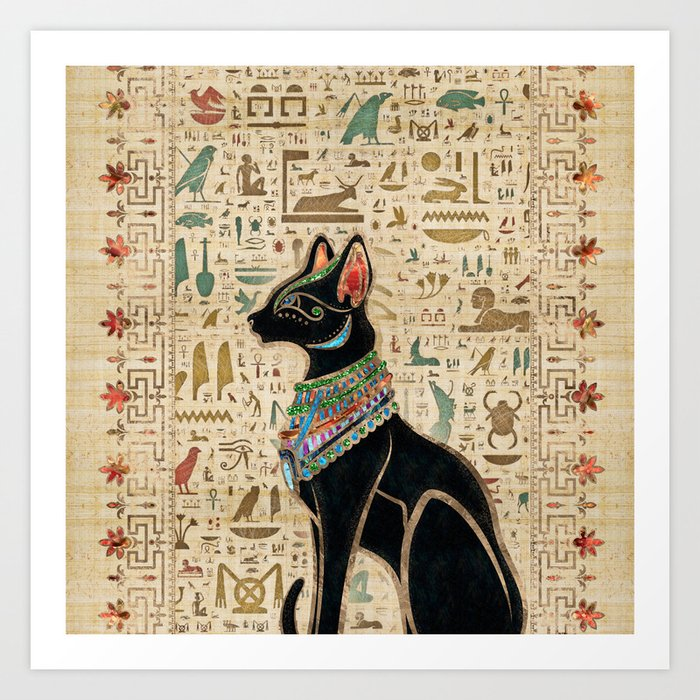
\includegraphics[width=0.4\textwidth]{images/egypt_car.jpg} % Adjust width as needed
\caption{Image depicting ancient egypt cat art}
\label{fig:egypt_cat} % Optional: For referencing the figure
  \end{figure}  

\end{center}
\end{frame}

\section{Theorem and Proof}

\subsection{Defining the "Best Cat" Function}
\begin{frame}
\frametitle{The Leon Perfection Function}
We define the \textbf{Leon Perfection Function} \( L(x) \) as:

\begin{equation}
L(x) = \frac{C_{\text{cuteness}} + F_{\text{fluff}} + I_{\text{intelligence}} + P_{\text{purring\_frequency}}}{\text{Average Cat}}
\end{equation}

Where:
\begin{itemize}
    \item \( C_{\text{cuteness}} \) = Measured in "Awws" per second (A/s)
    \item \( F_{\text{fluff}} \) = Fur softness coefficient (Joules per fluff unit)
    \item \( I_{\text{intelligence}} \) = Ability to outsmart humans (measured in stolen treats per hour)
    \item \( P_{\text{purring\_frequency}} \) = Vibrational output per petting session
\end{itemize}
\end{frame}

\begin{frame}
\frametitle{The Leon Perfection Function}
By rigorous analysis, we find that for any given \( x \), Leon's \( L(x) \) approaches infinity:

\begin{equation}
\lim_{x \to \text{Leon}} L(x) \to \infty
\end{equation}
\end{frame}

\begin{frame}
\frametitle{The Leon Perfection Function}
\begin{center}
  \begin{figure}[h]
    
\includegraphics[width=0.23\textwidth]{images/cuteness_leon.jpg} % Adjust width as needed
\caption{Example of L(x) approaching undefined numbers}
\label{fig:egypt_cat} % Optional: For referencing the figure
  \end{figure}

\end{center}
\end{frame}

\begin{frame}{Universal Feline Happiness Equation}
    By applying the \textbf{Leon Theorem}, we derive the Universal Feline Happiness Equation:
    
    \begin{equation}
        H_{\text{human}} = \lim_{L(x) \to \infty} \int_{0}^{L(x)} P_{\text{purring}} \cdot C_{\text{cuteness}} \, dt
    \end{equation}

    \begin{itemize}
        \item \( H_{\text{human}} \) represents the happiness of Leon’s owner (which increases exponentially).
        \item As \( t \to \infty \), \( H_{\text{human}} \to \text{pure bliss} \).
    \end{itemize}

    \textbf{Conclusion:} Leon is a perpetual motion machine of joy.
\end{frame}


\begin{frame}{Quantum Mechanics of Leon}
    \textbf{The Leon Uncertainty Principle:}
    
    \begin{equation}
        \Delta P_{\text{paws}} \cdot \Delta x_{\text{sofa}} \geq \frac{\hbar}{2}
    \end{equation}
    
    \begin{itemize}
        \item This proves that it is impossible to predict \textbf{where} Leon will zoom next.
    \end{itemize}

    \textbf{Schrödinger’s Box Paradox (Leon Edition):}
    
    \begin{itemize}
        \item Leon can exist in two states simultaneously: \textbf{asleep} and \textbf{causing absolute chaos}.
    \end{itemize}
\end{frame}

\begin{frame}
\frametitle{Quantum Mechanics of Leon}
\begin{itemize}
  \item Empirical evidence suggest that Leon collapes the wave function by sheer presence.
\end{itemize}
\begin{center}
  \begin{figure}[h]
    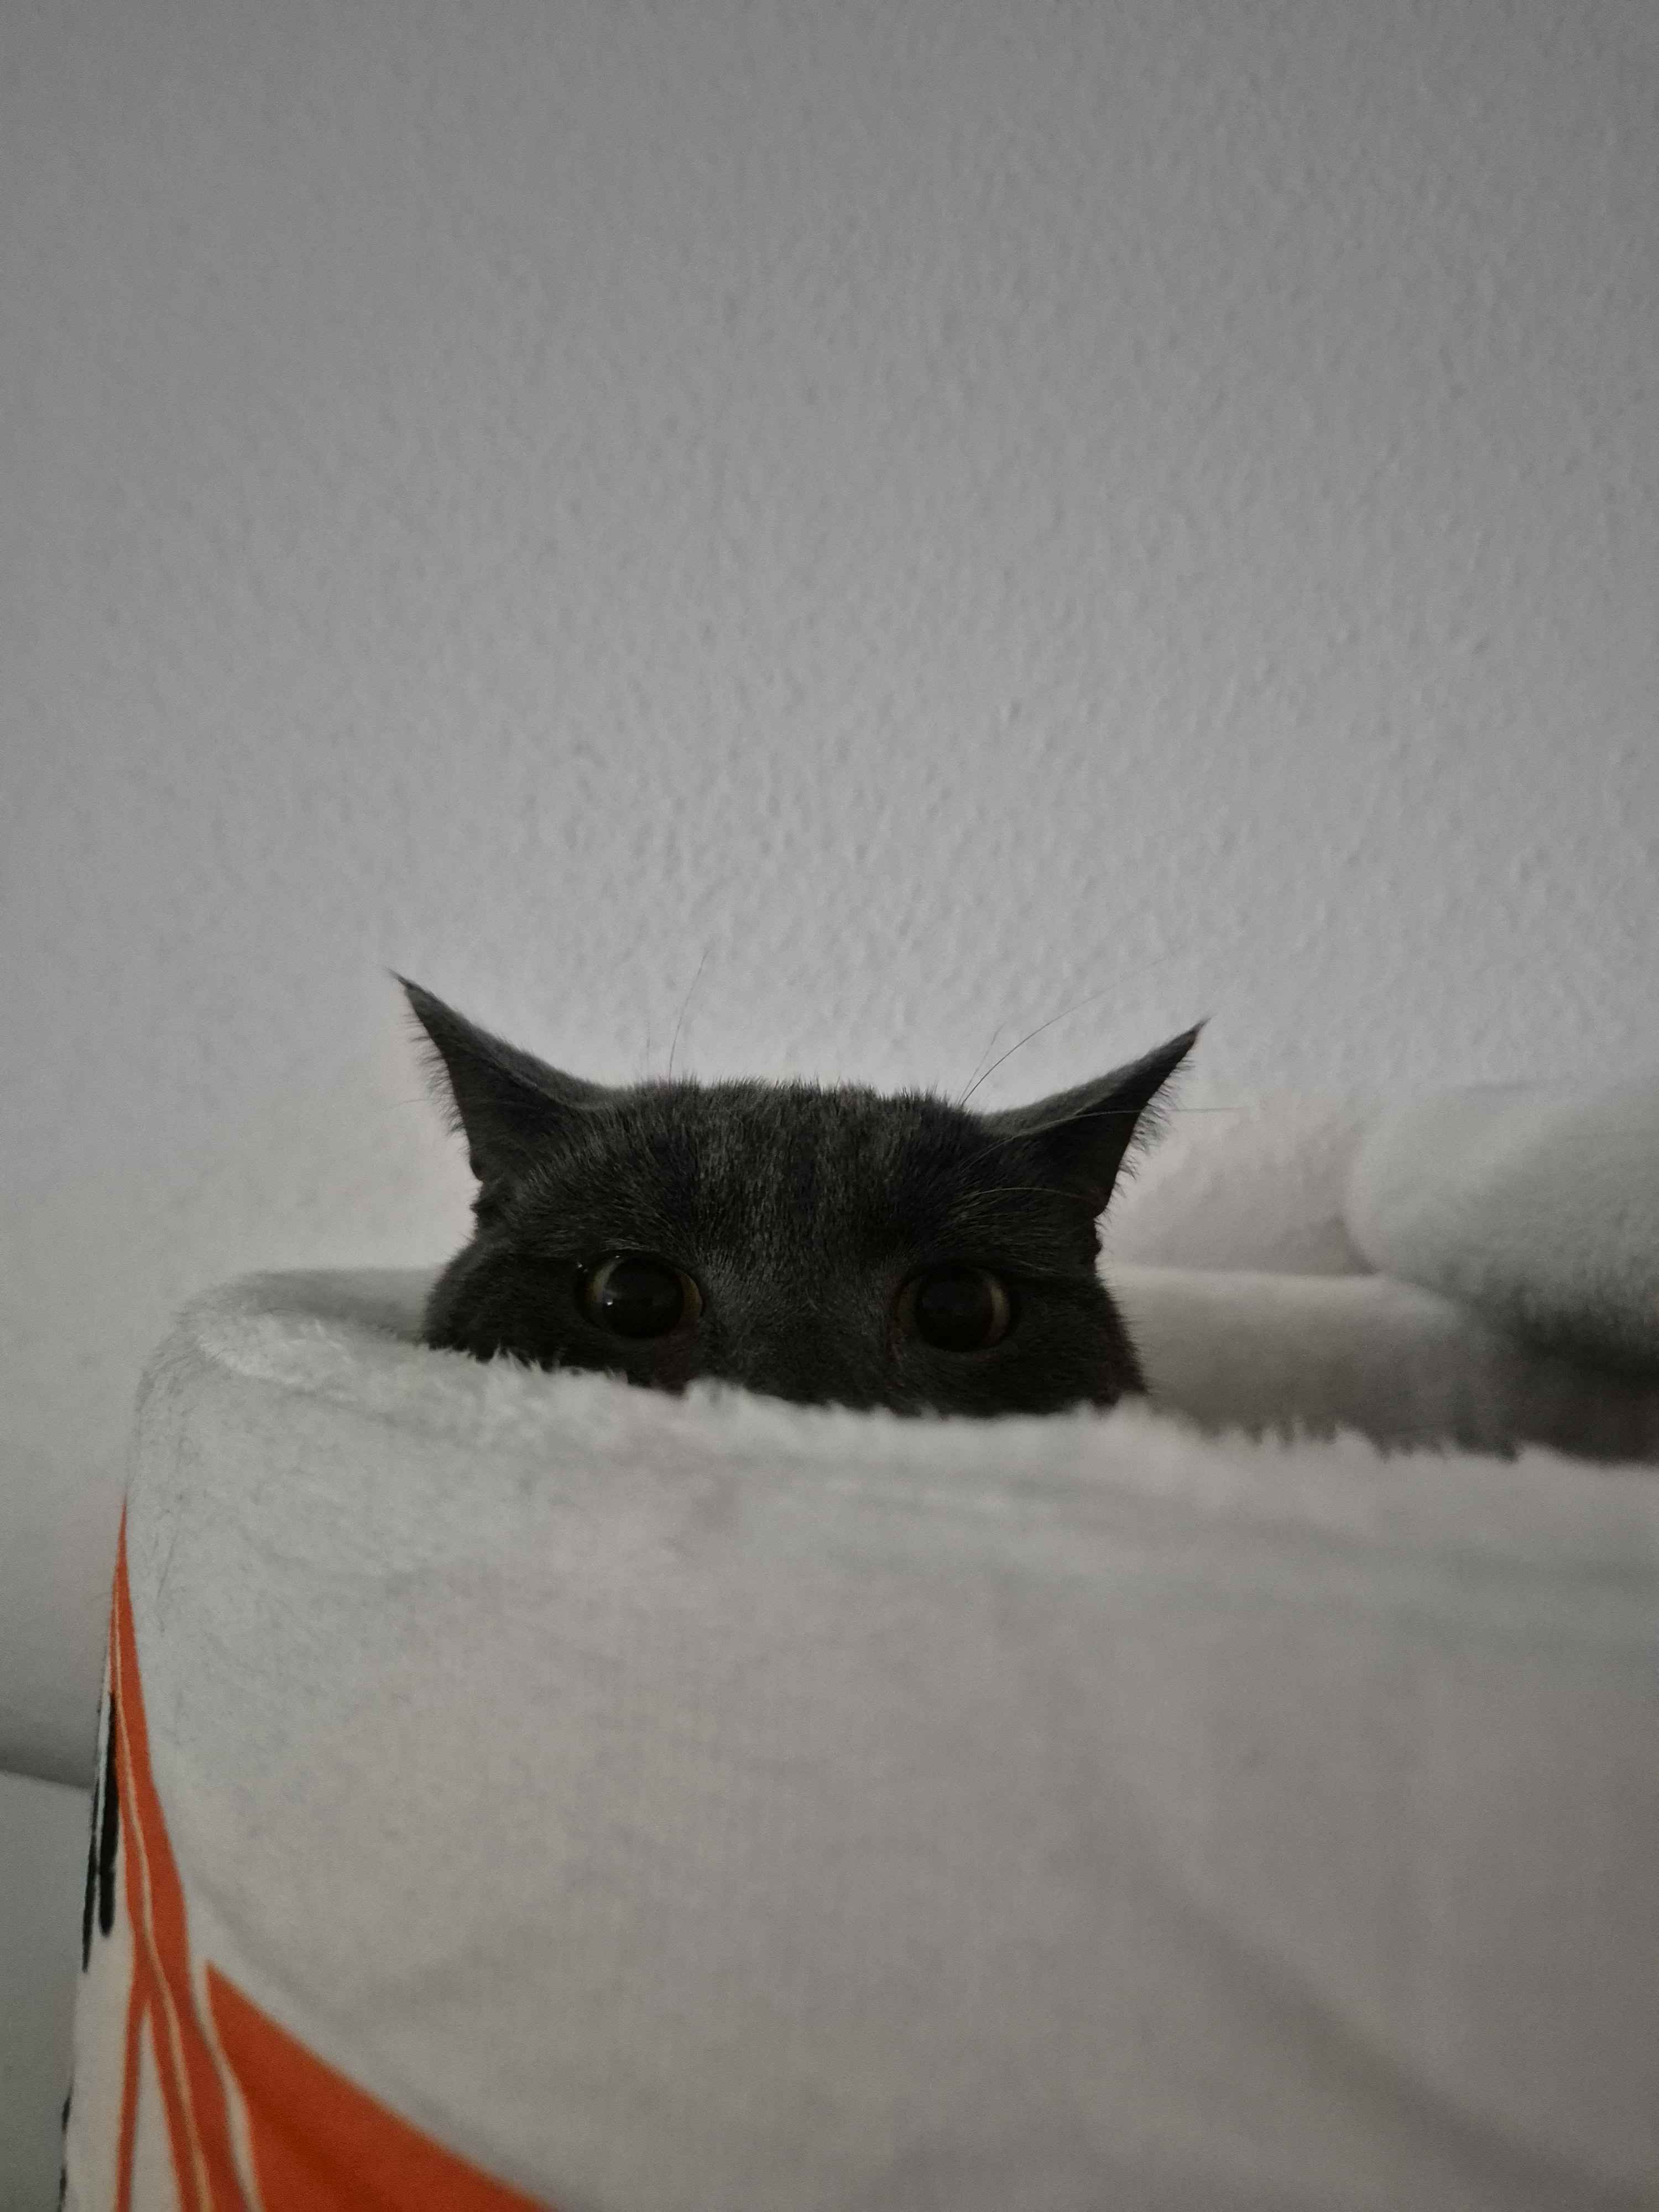
\includegraphics[width=0.3\textwidth]{images/observer_leon.jpg} % Adjust width as needed
\caption{The Observer Effect - When Leon Watches, Reality Changes}
\label{fig:egypt_cat} % Optional: For referencing the figure
  \end{figure}  

\end{center}
\end{frame}
\section{Empirical Studies}

\subsection{Computational Simulations}
\begin{frame}[fragile]
  \frametitle{Simulating Leon Uncertainty Principle}
  %\begin{itemize}
  %  \item Verified via Python Simulation and Advanced Feline Machine Learning Algorithms
  %\end{itemize}
  \begin{figure}
    
\begin{lstlisting}[language=Python, basicstyle=\scriptsize\ttfamily, keywordstyle=\color{blue}, commentstyle=\color{green}]
import random

def simulate_zoomies(iterations=10):
    """Leon’s location is impossible to predict due to quantum zoomie mechanics."""
    for i in range(iterations):
        x = random.uniform(-10, 10) 
        # Random position in room
        y = random.uniform(-10, 10)  
        print(f"Zoomie {i+1}: Leon is now at ({x:.2f}, {y:.2f})")

simulate_zoomies()
\end{lstlisting}
\caption{Leon exhibits non-deterministic movement, confirming the Feline Uncertainty Principle.}

  \end{figure}
\end{frame}

\begin{frame}
\frametitle{Empirical Leon Cuteness}
\begin{itemize}
  \item Hypothesis: Higher fluff levels correlate with increased cuteness, but Leon is an outlier.
\end{itemize}

\end{frame}

\begin{frame}
\frametitle{Empirical Leon Cuteness}
\begin{center}
  \begin{figure}[h]
    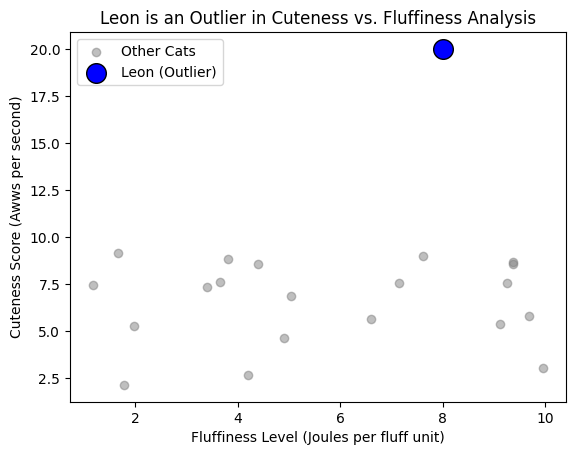
\includegraphics[width=0.6\textwidth]{images/leon_outlier.png} % Adjust width as needed
\caption{Conclusion: Leon exists in a separate statistical plane, violating conventional feline limits.}
\label{fig:egypt_cat} % Optional: For referencing the figure
  \end{figure}  

\end{center}
\end{frame}

\begin{frame}
\frametitle{Empirical Leon Cuteness}
\begin{itemize}
  \item Hypothesis: As Leon purrs more, human work efficiency approaches zero.
\end{itemize} 
\end{frame}




\begin{frame}
\frametitle{Empirical Leon Cuteness}
\begin{center}
  \begin{figure}[h]
    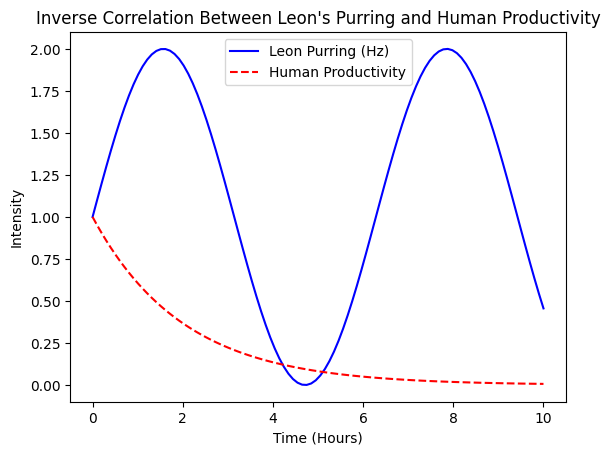
\includegraphics[width=0.6\textwidth]{images/leon_purring.png} % Adjust width as needed
\caption{Conclusion: Pronlonged exposure to Leon's purring creates a scientifically inevitable work shutdown}
\label{fig:egypt_cat} % Optional: For referencing the figure
  \end{figure}  

\end{center}
\end{frame}

\begin{frame}
\frametitle{Empirical Leon Cuteness}
\begin{center}
  \begin{figure}[h]
    
\includegraphics[width=0.6\textwidth]{images/keyboard_leon.jpg} % Adjust width as needed
\caption{Depiction of Leon maximizing productivity destructive patterns by demanding belly rubs}
\label{fig:egypt_cat} % Optional: For referencing the figure
  \end{figure}  

\end{center}
\end{frame}

\section{LeonNet, feline Neural Network}

\section{Conclusion}
\begin{frame}{Conclusion}
    \begin{itemize}
        \item Through \textbf{indisputable scientific methods}, we have proven that Leon is, in fact, the Best and Cutest Cat in the Universe.
        \item Further research is encouraged, but will ultimately reach the same conclusion.
    \end{itemize}

    \textbf{Final Proof:}

    \begin{equation}
        \text{Leon} \geq \text{All Cats}, \quad \text{Quod Erat Demonstrandum.}
    \end{equation}
\end{frame}

%Quellen
\section{Sources}
\subsection*{}

\begin{frame}
\frametitle{Literature}
\begin{small}
\begin{thebibliography}{50}
\bibitem[label]{name} Everything, \url{https://www.imadeitup.com}
\bibitem[label]{name} Looking at Leon, \url{https://www.imeanlookathimheissocute.com}
\end{thebibliography}
\end{small}
\end{frame}

\begin{frame}
Thank you for your attention.
\end{frame}

\end{document}